% 作者:Anders Sjoqvist 与 Ulf Lundstrom,2009
% 主要来源:tinyKACTL、Beta 与 Wikipedia

\chapter{数学}

\section{方程}
\[ax^2+bx+c=0 \Rightarrow x = \frac{-b\pm\sqrt{b^2-4ac}}{2a}\]

极值点为 $x = -b/2a$。

\[\begin{aligned}ax+by=e\\cx+dy=f\end{aligned}
\Rightarrow
\begin{aligned}x=\dfrac{ed-bf}{ad-bc}\\y=\dfrac{af-ec}{ad-bc}\end{aligned}\]

一般地,给定方程 $Ax = b$,变量 $x_i$ 的解为
\[x_i = \frac{\det A_i'}{\det A} \]
其中 $A_i'$ 是把 $A$ 的第 $i$ 列换成 $b$ 所得的矩阵。

\section{递推}
若 $a_n = c_1 a_{n-1} + \dots + c_k a_{n-k}$,$r_1, \dots, r_k$ 是 $x^k - c_1 x^{k-1} - \dots - c_k$ 的互异根,则存在 $d_1, \dots, d_k$ 使
\[a_n = d_1r_1^n + \dots + d_kr_k^n. \]
重根 $r$ 变为多项式因子,如 $a_n = (d_1n + d_2)r^n$。

\section{三角}
\begin{align*}
\sin(v+w)&{}=\sin v\cos w+\cos v\sin w\\
\cos(v+w)&{}=\cos v\cos w-\sin v\sin w\\
\end{align*}
\begin{align*}
\tan(v+w)&{}=\dfrac{\tan v+\tan w}{1-\tan v\tan w}\\
\sin v+\sin w&{}=2\sin\dfrac{v+w}{2}\cos\dfrac{v-w}{2}\\
\cos v+\cos w&{}=2\cos\dfrac{v+w}{2}\cos\dfrac{v-w}{2}
\end{align*}
\[ (V+W)\tan(v-w)/2{}=(V-W)\tan(v+w)/2 \]
其中 $V, W$ 为角 $v, w$ 所对边长。
\begin{align*}
	a\cos x+b\sin x&=r\cos(x-\phi)\\
	a\sin x+b\cos x&=r\sin(x+\phi)
\end{align*}
其中 $r=\sqrt{a^2+b^2}, \phi=\operatorname{atan2}(b,a)$。

\section{几何}

\subsection{三角形}
边长:$a,b,c$\\
半周长:$p=\dfrac{a+b+c}{2}$\\
面积:$A=\sqrt{p(p-a)(p-b)(p-c)}$\\
外接圆半径:$R=\dfrac{abc}{4A}$\\
内切圆半径:$r=\dfrac{A}{p}$\\
中线长(把三角形分成两个等面积三角形):$m_a=\tfrac{1}{2}\sqrt{2b^2+2c^2-a^2}$\\
角平分线长(把角平分):$s_a=\sqrt{bc\left[1-\left(\dfrac{a}{b+c}\right)^2\right]}$\\
正弦定理:$\dfrac{\sin\alpha}{a}=\dfrac{\sin\beta}{b}=\dfrac{\sin\gamma}{c}=\dfrac{1}{2R}$\\
余弦定理:$a^2=b^2+c^2-2bc\cos\alpha$\\
正切定理:$\dfrac{a+b}{a-b}=\dfrac{\tan\dfrac{\alpha+\beta}{2}}{\tan\dfrac{\alpha-\beta}{2}}$\\

\subsection{四边形}
边长 $a,b,c,d$,对角线 $e, f$,对角线夹角 $\theta$,面积 $A$,以及
魔法量 $F=b^2+d^2-a^2-c^2$:

\[ 4A = 2ef \cdot \sin\theta = F\tan\theta = \sqrt{4e^2f^2-F^2} \]

 对圆内接四边形,对角之和为 $180^\circ$,
$ef = ac + bd$,且 $A = \sqrt{(p-a)(p-b)(p-c)(p-d)}$。

\subsection{球坐标}
\begin{center}
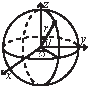
\includegraphics[width=25mm]{content/math/sphericalCoordinates}
\end{center}
\[\begin{array}{cc}
x = r\sin\theta\cos\phi & r = \sqrt{x^2+y^2+z^2}\\
y = r\sin\theta\sin\phi & \theta = \textrm{acos}(z/\sqrt{x^2+y^2+z^2})\\
z = r\cos\theta & \phi = \textrm{atan2}(y,x)
\end{array}\]

\section{导数与积分}
\begin{align*}
	\dfrac{d}{dx}\arcsin x = \dfrac{1}{\sqrt{1-x^2}} &&& \dfrac{d}{dx}\arccos x = -\dfrac{1}{\sqrt{1-x^2}} \\
	\dfrac{d}{dx}\tan x = 1+\tan^2 x &&& \dfrac{d}{dx}\arctan x = \dfrac{1}{1+x^2} \\
	\int\tan ax = -\dfrac{\ln|\cos ax|}{a} &&& \int x\sin ax = \dfrac{\sin ax-ax \cos ax}{a^2} \\
	\int e^{-x^2} = \frac{\sqrt \pi}{2} \text{erf}(x) &&& \int xe^{ax}dx = \frac{e^{ax}}{a^2}(ax-1)
\end{align*}

分部积分:
\[\int_a^bf(x)g(x)dx = [F(x)g(x)]_a^b-\int_a^bF(x)g'(x)dx\]

\section{求和}
\[ c^a + c^{a+1} + \dots + c^{b} = \frac{c^{b+1} - c^a}{c-1}, c \neq 1 \]
\begin{align*}
	1 + 2 + 3 + \dots + n &= \frac{n(n+1)}{2} \\
	1^2 + 2^2 + 3^2 + \dots + n^2 &= \frac{n(2n+1)(n+1)}{6} \\
	1^3 + 2^3 + 3^3 + \dots + n^3 &= \frac{n^2(n+1)^2}{4} \\
	1^4 + 2^4 + 3^4 + \dots + n^4 &= \frac{n(n+1)(2n+1)(3n^2 + 3n - 1)}{30} \\
\end{align*}

\section{级数}
$$e^x = 1+x+\frac{x^2}{2!}+\frac{x^3}{3!}+\dots,\,(-\infty<x<\infty)$$
$$\ln(1+x) = x-\frac{x^2}{2}+\frac{x^3}{3}-\frac{x^4}{4}+\dots,\,(-1<x\leq1)$$
$$\sqrt{1+x} = 1+\frac{x}{2}-\frac{x^2}{8}+\frac{2x^3}{32}-\frac{5x^4}{128}+\dots,\,(-1\leq x\leq1)$$
$$\sin x = x-\frac{x^3}{3!}+\frac{x^5}{5!}-\frac{x^7}{7!}+\dots,\,(-\infty<x<\infty)$$
$$\cos x = 1-\frac{x^2}{2!}+\frac{x^4}{4!}-\frac{x^6}{6!}+\dots,\,(-\infty<x<\infty)$$

\section{概率论}
设 $X$ 为离散随机变量,取值 $x$ 的概率为 $p_X(x)$。则其期望(均值)为 $\mu=\mathbb{E}(X)=\sum_xxp_X(x)$,方差为 $\sigma^2=V(X)=\mathbb{E}(X^2)-(\mathbb{E}(X))^2=\sum_x(x-\mathbb{E}(X))^2p_X(x)$,其中 $\sigma$ 为标准差。若 $X$ 是连续的,则有概率密度函数 $f_X(x)$,上面的求和相应变为积分,并把 $p_X(x)$ 换成 $f_X(x)$。

期望是线性的:
\[\mathbb{E}(aX+bY) = a\mathbb{E}(X)+b\mathbb{E}(Y)\]
对独立的 $X$ 与 $Y$,\[V(aX+bY) = a^2V(X)+b^2V(Y).\]

\subsection{离散分布}

\subsubsection{二项分布}
$n$ 次独立的是/否实验中,每次成功概率为 $p$,成功次数服从 $\textrm{Bin}(n,p),\,n=1,2,\dots,\, 0\leq p\leq1$。
\[p(k)=\binom{n}{k}p^k(1-p)^{n-k}\]
\[\mu = np,\,\sigma^2=np(1-p)\]
$p$ 较小时,$\textrm{Bin}(n,p)$ 近似为 $\textrm{Po}(np)$。

\subsubsection{首次成功分布}
独立的是/否实验中,首次成功所需的实验次数服从 $\textrm{Fs}(p),\,0\leq p\leq1$。
\[p(k)=p(1-p)^{k-1},\,k=1,2,\dots\]
\[\mu = \frac1p,\,\sigma^2=\frac{1-p}{p^2}\]

\subsubsection{泊松分布}
固定时间 $t$ 内发生的事件数,若事件以已知平均速率 $\kappa$ 发生且与上次事件后经过的时间无关,则服从 $\textrm{Po}(\lambda),\,\lambda=t\kappa$。
\[p(k)=e^{-\lambda}\frac{\lambda^k}{k!}, k=0,1,2,\dots\]
\[\mu=\lambda,\,\sigma^2=\lambda\]

\subsection{连续分布}

\subsubsection{均匀分布}
概率密度函数在 $a$ 与 $b$ 之间为常数、其余为 0 时,服从 $\textrm{U}(a,b),\,a<b$。
\[f(x) = \left\{
\begin{array}{cl}
\frac{1}{b-a} & a<x<b\\
0 & \textrm{其它}
\end{array}\right.\]
\[\mu=\frac{a+b}{2},\,\sigma^2=\frac{(b-a)^2}{12}\]

\subsubsection{指数分布}
泊松过程中两次事件之间的时间服从 $\textrm{Exp}(\lambda),\,\lambda>0$。
\[f(x) = \left\{
\begin{array}{cl}
\lambda e^{-\lambda x} & x\geq0\\
0 & x<0
\end{array}\right.\]
\[\mu=\frac{1}{\lambda},\,\sigma^2=\frac{1}{\lambda^2}\]

\subsubsection{正态分布}
大多数均值为 $\mu$、方差为 $\sigma^2$ 的实际随机值都可由 $\mathcal{N}(\mu,\sigma^2),\,\sigma>0$ 很好地描述。
\[ f(x) = \frac{1}{\sqrt{2\pi\sigma^2}}e^{-\frac{(x-\mu)^2}{2\sigma^2}} \]
若 $X_1 \sim \mathcal{N}(\mu_1,\sigma_1^2)$ 且 $X_2 \sim \mathcal{N}(\mu_2,\sigma_2^2)$,则
\[ aX_1 + bX_2 + c \sim \mathcal{N}(\mu_1+\mu_2+c,a^2\sigma_1^2+b^2\sigma_2^2) \]

\section{马尔可夫链}
\emph{马尔可夫链}是一种离散随机过程,其性质是下一状态只依赖当前状态。
设 $X_1,X_2,\ldots$ 为马尔可夫过程生成的随机变量序列。
则存在转移矩阵 $\mathbf{P} = (p_{ij})$,$p_{ij} = \Pr(X_n = i | X_{n-1} = j)$,
且 $\mathbf{p}^{(n)} = \mathbf P^n \mathbf p^{(0)}$ 是 $X_n$ 的概率分布(即 $p^{(n)}_i = \Pr(X_n = i)$),
其中 $\mathbf{p}^{(0)}$ 是初始分布。

% \subsubsection{平稳分布}
$\mathbf{\pi}$ 是平稳分布,若 $\mathbf{\pi} = \mathbf{\pi P}$。
若马尔可夫链\emph{不可约}(从任意状态可到达任意状态),
则 $\pi_i = \frac{1}{\mathbb{E}(T_i)}$,其中 $\mathbb{E}(T_i)$ 是两次访问状态 $i$ 之间的期望时间。
$\pi_j/\pi_i$ 是两次访问状态 $i$ 之间访问状态 $j$ 的期望次数。

对连通、无向、非二分图,转移概率在所有邻居间均匀时,$\pi_i$ 正比于节点 $i$ 的度数。

% \subsubsection{遍历性}
马尔可夫链是\emph{遍历的},若其渐近分布与初始分布无关。
有限马尔可夫链遍历当且仅当其不可约且\emph{非周期}(即所有环长的 gcd 为 1)。
$\lim_{k\rightarrow\infty}\mathbf{P}^k = \mathbf{1}\pi$。

% \subsubsection{吸收}
马尔可夫链是 A-链,若状态可分为 $\mathbf{A}$ 与 $\mathbf{G}$ 两组,
使 $\mathbf{A}$ 中所有状态都是吸收态($p_{ii}=1$),且 $\mathbf{G}$ 中所有状态都通向 $\mathbf{A}$ 中的吸收态。
初始状态为 $j$ 时,在状态 $i\in\mathbf{A}$ 被吸收的概率为 $a_{ij} = p_{ij}+\sum_{k\in\mathbf{G}} a_{ik}p_{kj}$。
初始状态为 $i$ 时,到吸收的期望时间为 $t_i = 1+\sum_{k\in\mathbf{G}}p_{ki}t_k$。
